
%
%
% Module: surround_sound_processor_exercise
%
% Author: Swaroop Appadwedula
%
%

Implement the passive decoder shown in Figure \ref{fig:decoder} on
the DSP.  Use an appropriate time delay based on the distance
between the front and back speakers, and the speed of sound.

\begin{figure}[htb]
    \begin{center}
	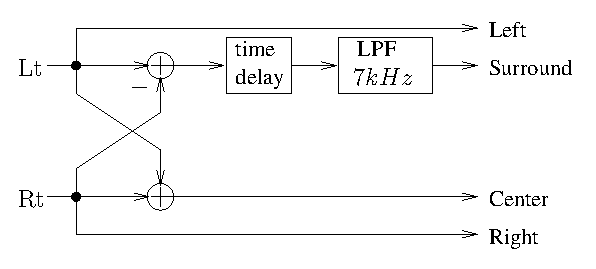
\epsfig{file=decoder.eps,width=8cm}
	\vspace*{0.5cm}
	\caption{Dolby Pro Logic Passive Decoder}
	\label{fig:decoder}
    \end{center}
\end{figure}

Is there significant crosstalk between the front and surround
speakers?  Do you get good separation between left and right
speakers?  How could power levels in the different channels be
used to provide directional enhancement?

For active decoding, you may consider using a Chamberlin filter
(see Chamberlin filter handout).  One way to find the power level
in a signal is to square it and pass it through a very narrow-band low-pass
filter ($\le 80 Hz$).
Squaring a signal in the time domain is equivalent to convolving
the signal with itself in the frequency domain.  In the frequency
domain, the resulting convolved signal near zero frequency corresponds
to the area under the original signal.

